\subsubsection{Kinematically-driven 2d oceanic subduction}
\label{sec:cookbooks-kinematic-2d-oceanic-subduction}

\textit{This section was contributed by Anne Glerum.}

This subduction example is based on the benchmark effort of Quinquis et al., of which initial results were published in \cite{Quinquis2014}. In four increasingly complex setups we will go from isoviscous materials without any temperature effects to a fully thermo-mechanical, nonlinear, strain-weakened visco-plastic, externally-driven model of oceanic subduction. The setup of the most complex case is outlined in Fig.~\ref{fig:QQ_setup}. The models are run for 15 My and slab tip depth, trench location, RMS velocity and temperature, and viscous dissipation are monitored. In addition, we discuss the effects of the element size of the subduction interface and crustal layers, viscosity averaging and the solver tolerance.

\begin{figure}
    \centering
    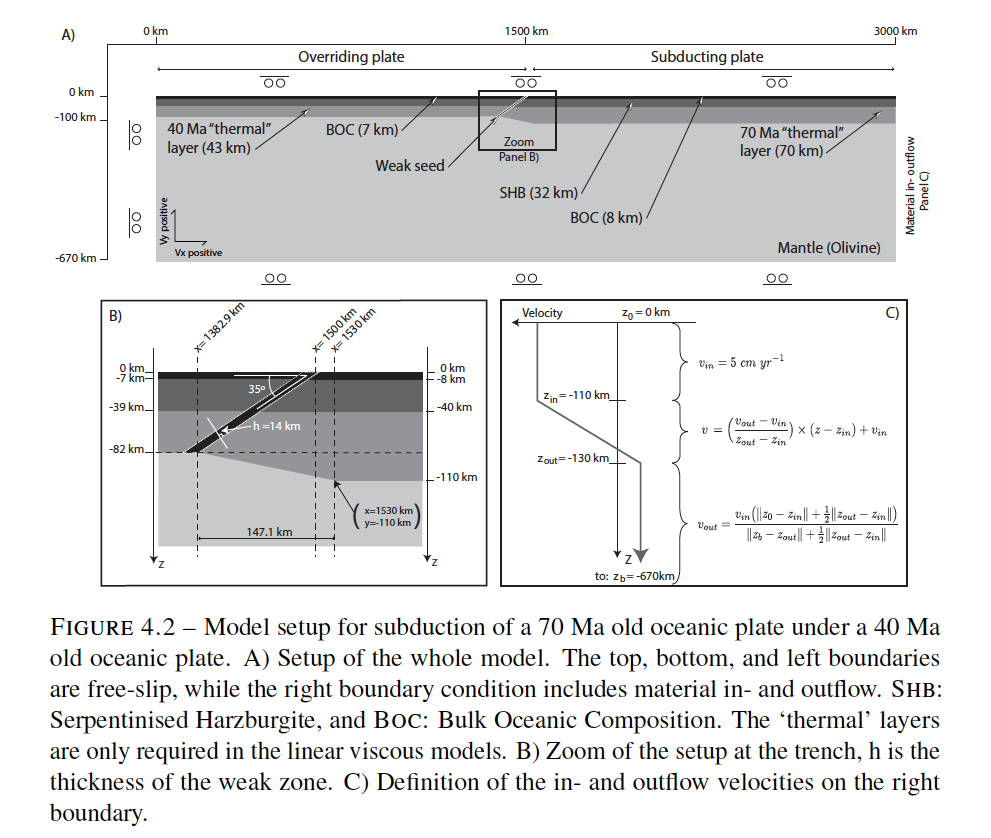
\includegraphics[width=0.8\textwidth]{setup_Quinquis2014.png}
    \caption{Case 4 model setup. Copied from Quinquis (2014).}
    \label{fig:QQ_setup}
\end{figure}

\paragraph{Case 1: Simple geometry and rheology}
The Case 1 model setup considers three materials (compositional fields) apart from the background sublithospheric mantle (see Fig.~\ref{fig:QQ_case1_setup}): 
\begin{enumerate}
    \item the lithosphere of the overriding plate (combining the BOC, SHB and thermal layer of the overriding plate in Fig.~\ref{fig:QQ_setup}),
    \item the crust of the subducting plate (weak seed and BOC combined), and
    \item the mantle lithosphere of the subducting plate (SHB and thermal layer combined).
\end{enumerate}{}
The geometry of these compositions is implemented as follows:
\lstinputlisting[language=prmfile]{Case1_compositions.prm.out}

No differences in material properties exist, except for density and viscosity, so we use the multicomponent material model. To keep the boundaries between fields as sharp as possible in terms of viscosity, we use the maximum composition to determine the viscosity in each evaluation point (note that this can be harder on the solver):
\lstinputlisting[language=prmfile]{Case1_materialmodel.prm.out}

Temperature effects are ignored. Subduction is driven by prescribed in- and outflow through the right boundary (with a gradual transition of the flow direction), all other boundaries are free slip. The volume of material that flows in is balanced by the volume that is prescribed to flow out (this is important as the model is incompressible). A weak crust along the plate interface and the subducting lithosphere facilitates subduction. Through the function plugin, we prescribe the in- and outflow:
\lstinputlisting[language=prmfile]{Case1_velocity.prm.out}

To follow the slab on its descent into the mantle, we use adaptive mesh refinement based on viscosity in combination with the minimum refinement strategy to ensure sufficient resolution in the crust and weak zone that allow the slab to detach from the surface:
\lstinputlisting[language=prmfile]{Case1_meshrefinement.prm.out}

To monitor the model evolution, several diagnostic quantities are tracked over time: the depth of the tip of the slab, the position of the trench, the RMS velocity of the slab and the whole model domain, and the work done (viscous dissipation) in the slab and total model domain. The computation of these quantities in done in several new plugins:
\lstinputlisting[language=prmfile]{Case1_postprocessing.prm.out}

\begin{figure}
    \centering
    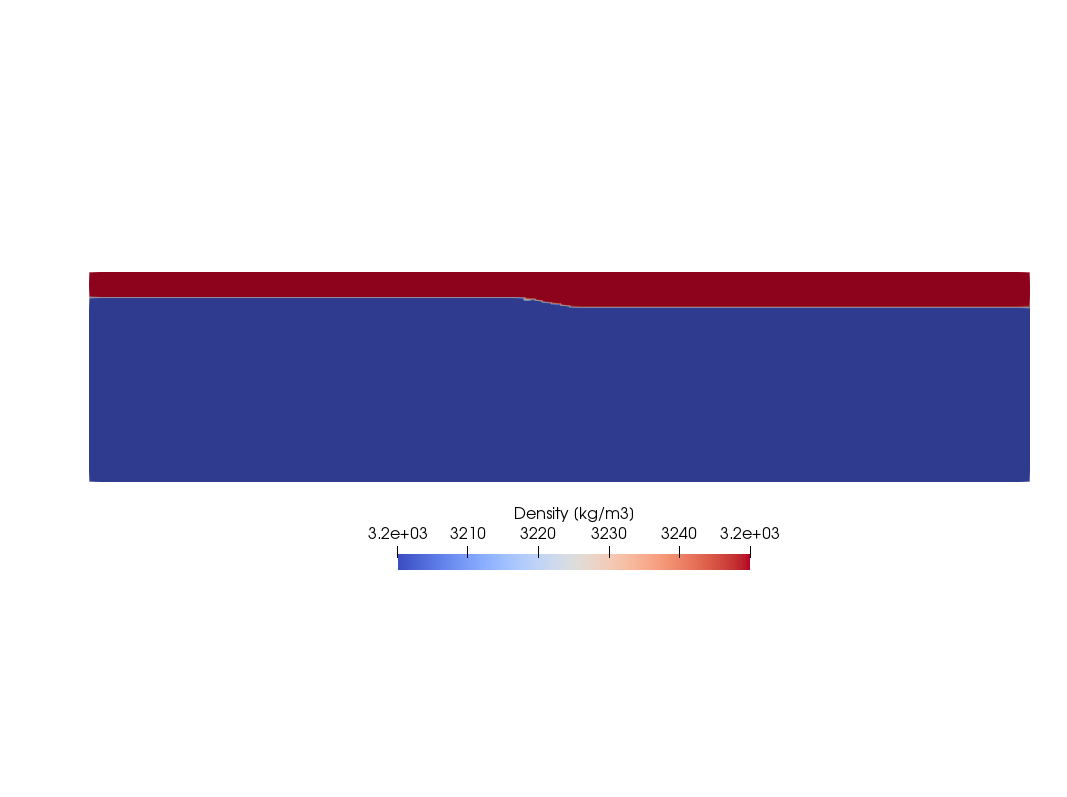
\includegraphics[width=0.6\textwidth,trim=1cm 7cm 1cm 8cm, clip=true]{Case1_dens_t0.png}
    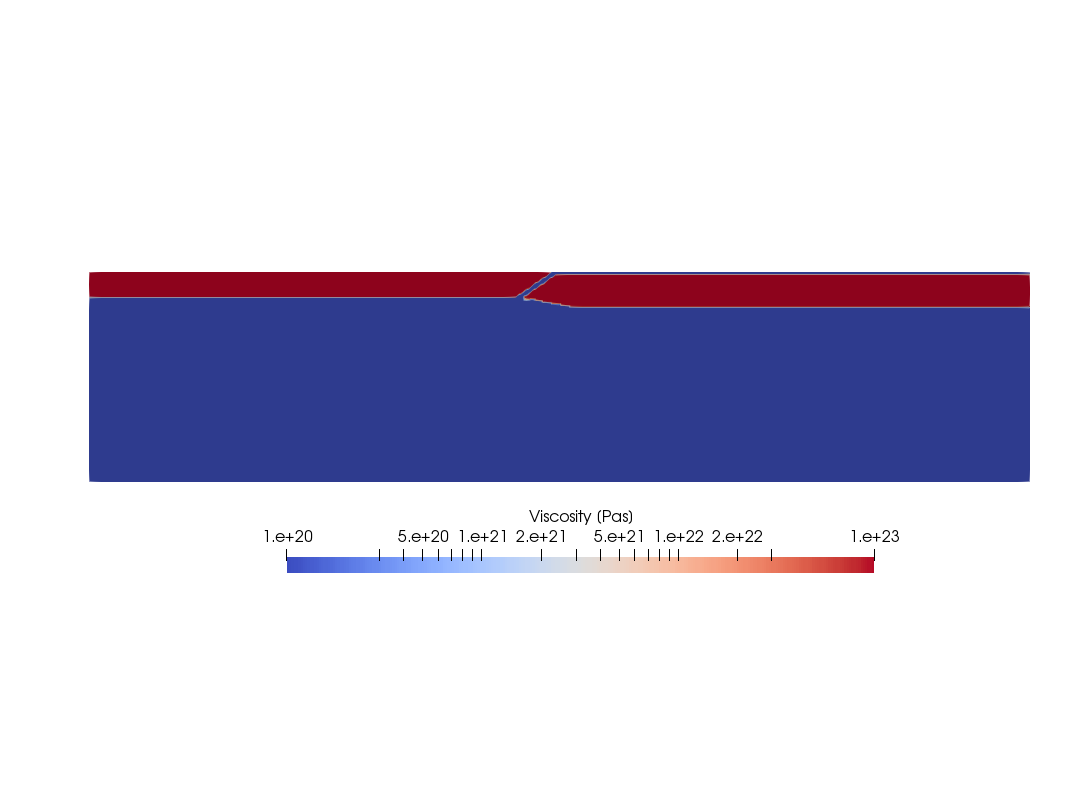
\includegraphics[width=0.6\textwidth,trim=1cm 7cm 1cm 8cm, clip=true]{Case1_visc_t0.png}
    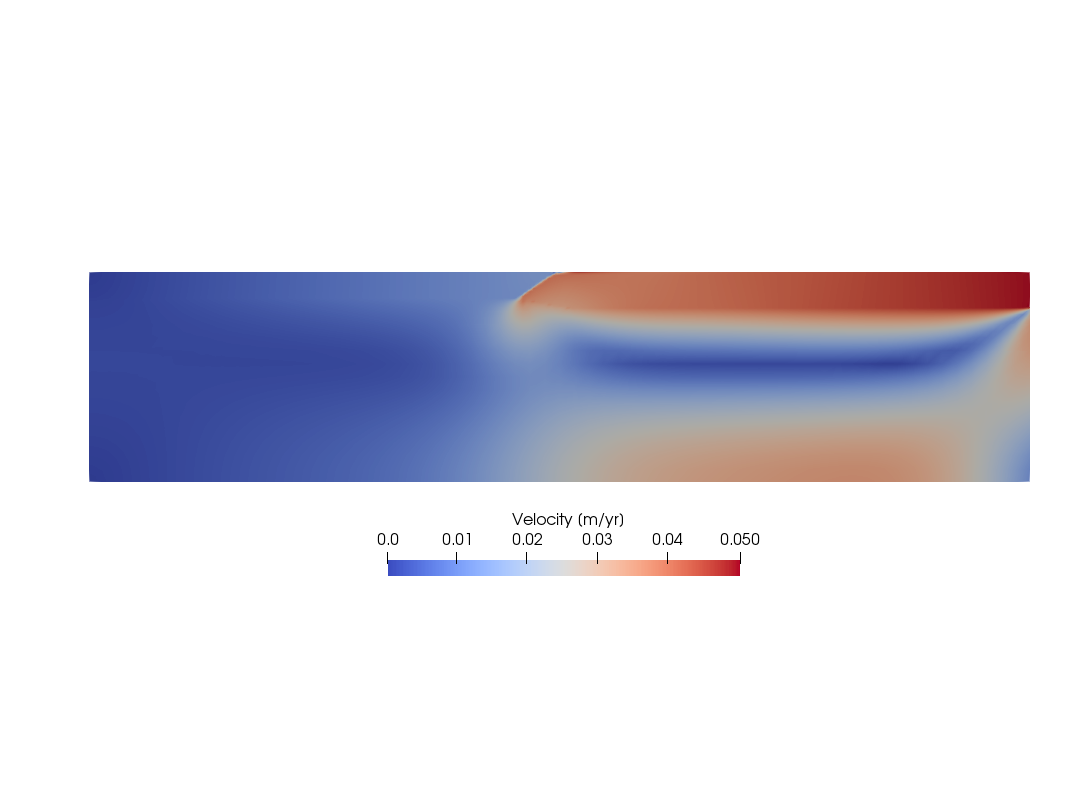
\includegraphics[width=0.6\textwidth,trim=1cm 7cm 1cm 8cm, clip=true]{Case1_vel_t0.png}
    \caption{\it Case 1 density, viscosity and velocity at time zero.}
    \label{fig:QQ_case1_setup}
\end{figure}

We run the Case 1 setup for 15 My of model time. The diagnostic quantities in Fig.~\ref{fig:QQ_case1_diagnostics} show three stages of model evolution: first trench advance (top right plot), then free subduction (increasing slab RMS velocity), and after about 13 My interaction between the slab and bottom boundary at 660 km depth, which slows down the slab. The slab then curves inward along the bottom boundary. This can also be seen in Fig~\ref{fig:QQ_case1_results}.

\begin{figure}
    \centering
    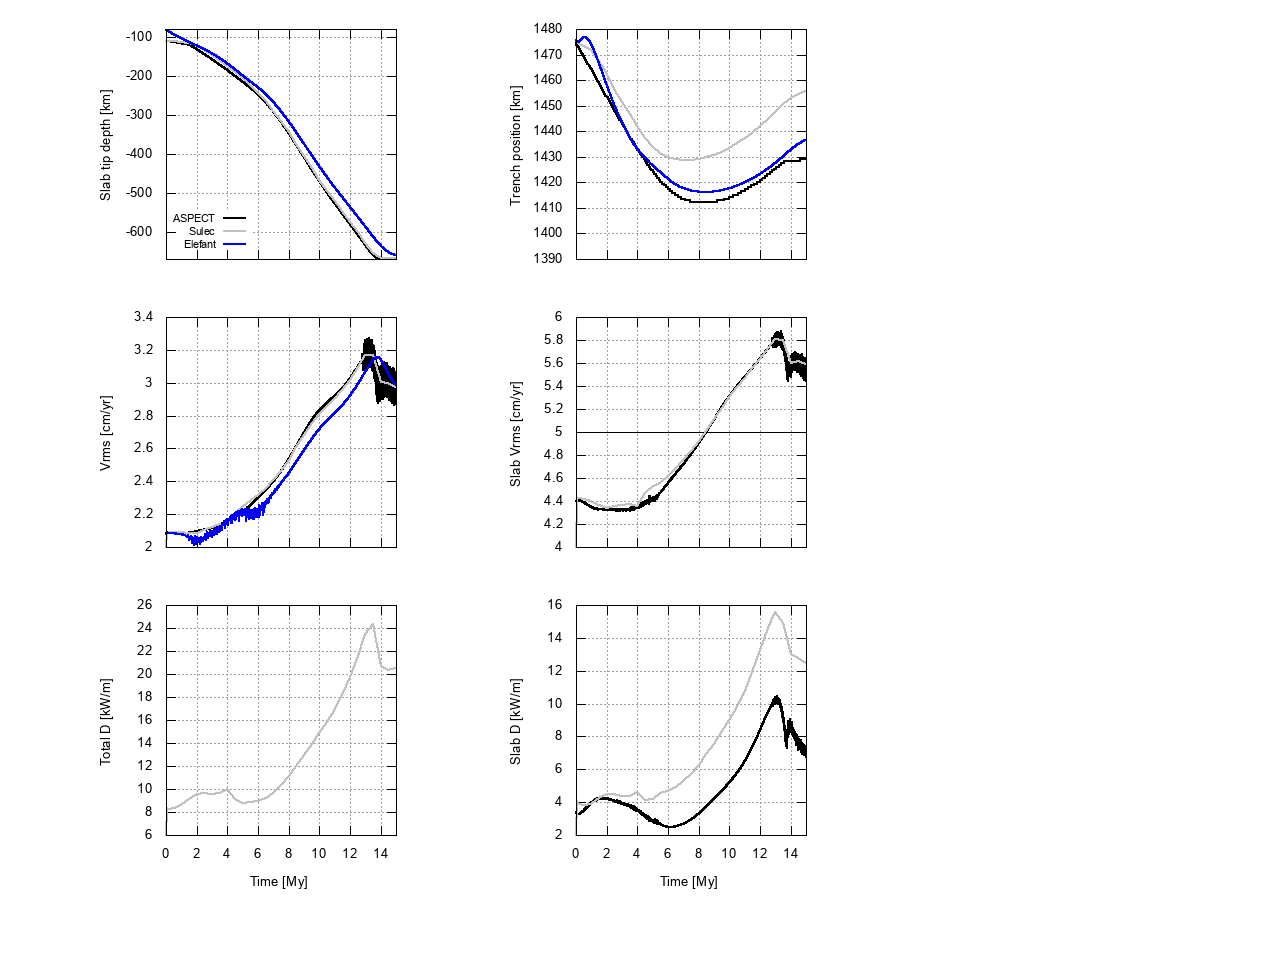
\includegraphics[trim=1cm 1cm 10cm 0cm,width=.8\textwidth]{Case1_diagnostics}
    \caption{\it Case 1 diagnostic quantities of ASPECT, Sulec and Elefant results.}
    \label{fig:QQ_case1_diagnostics}
\end{figure}

\begin{figure}
    \centering
    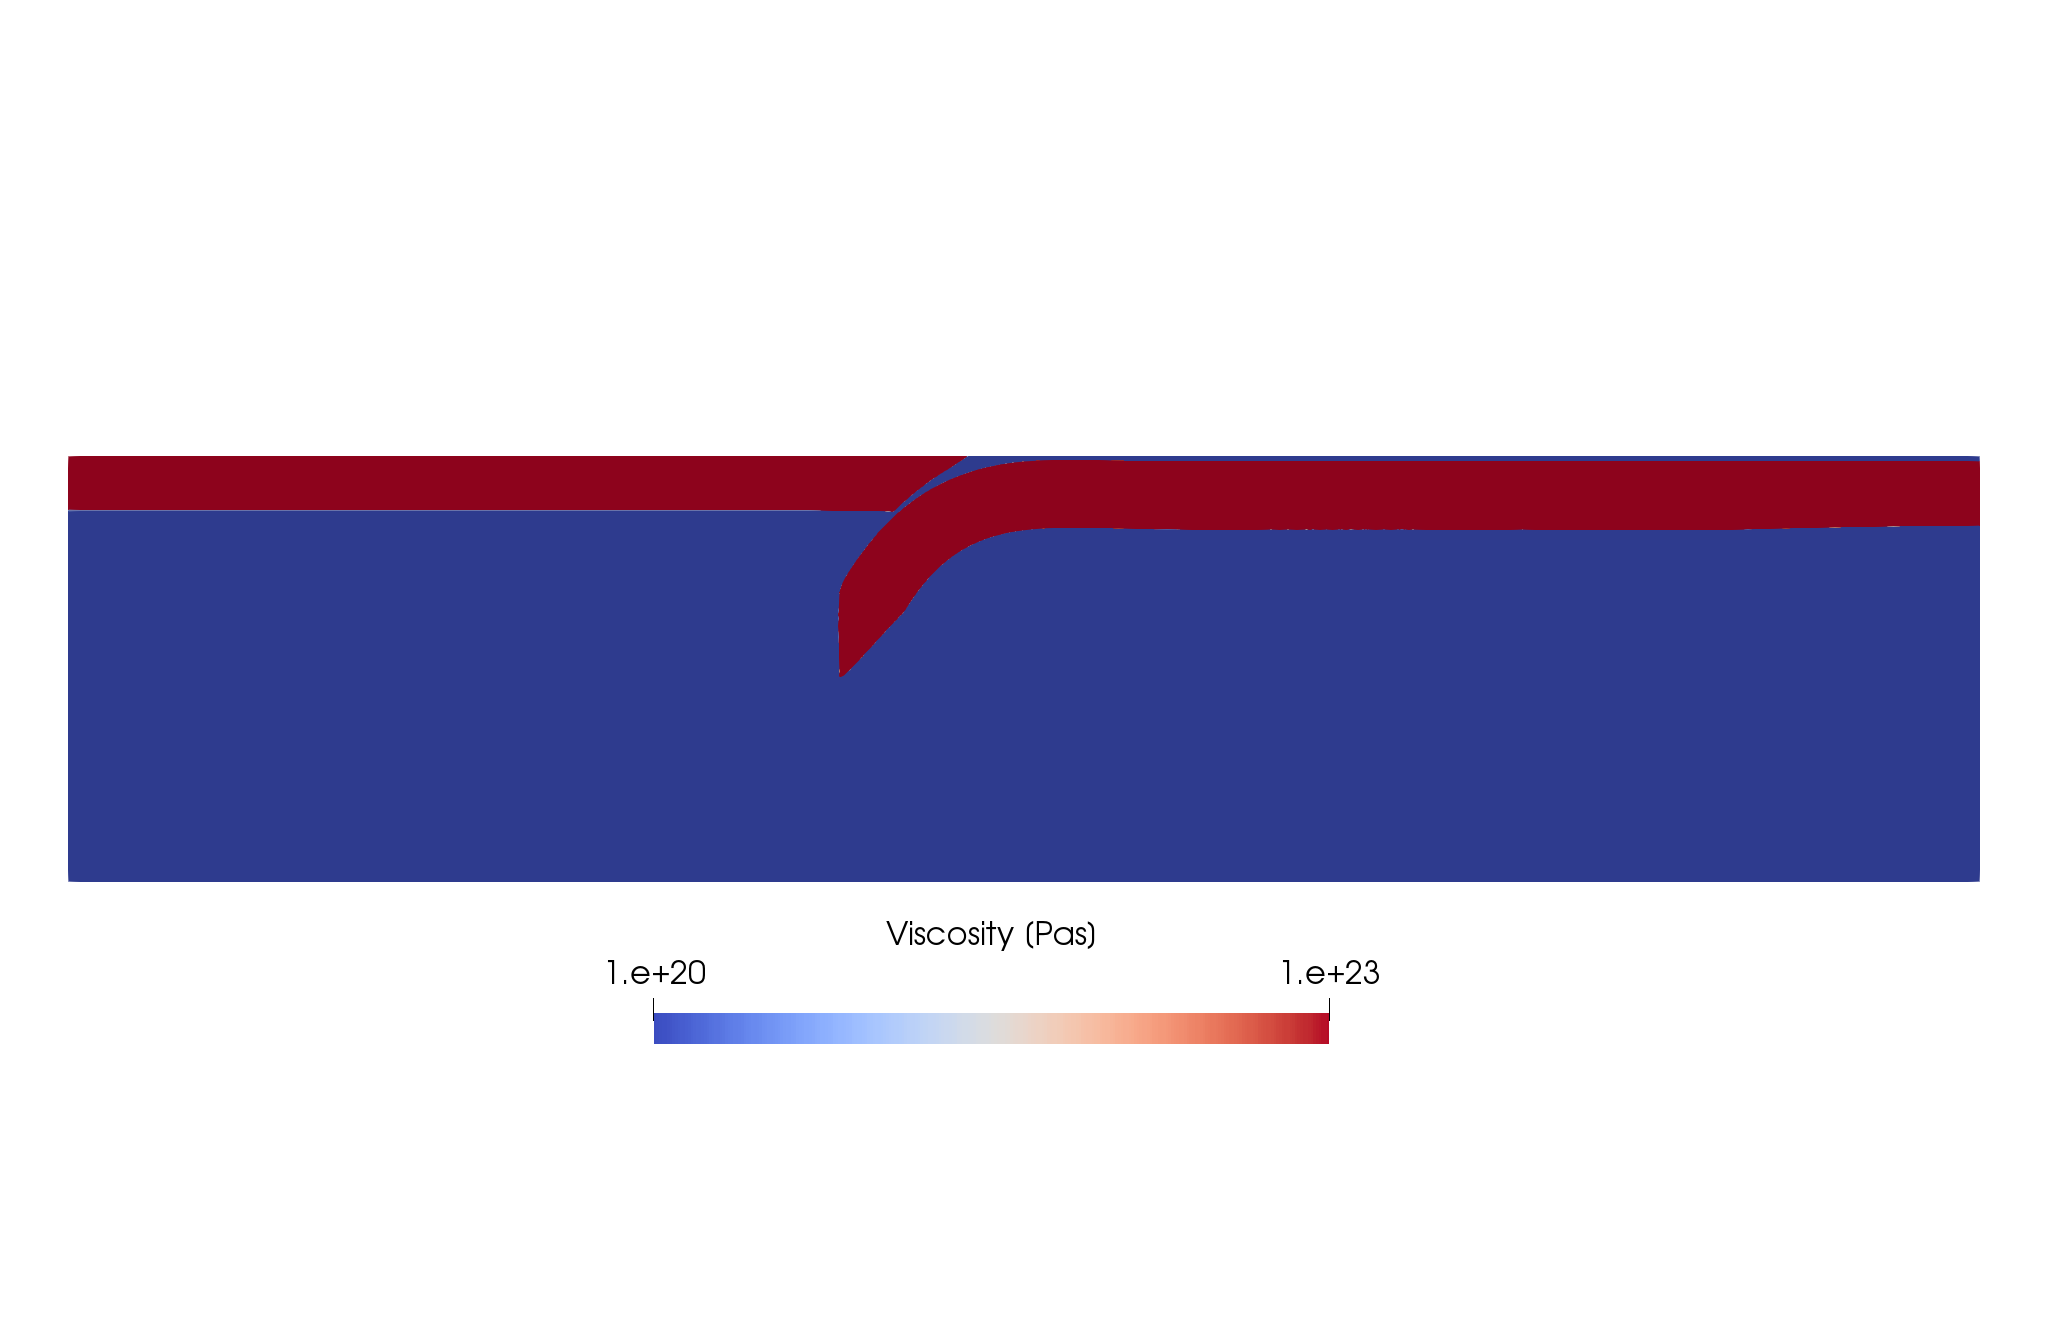
\includegraphics[width=0.6\textwidth,trim=1cm 10cm 1cm 9cm, clip=true]{Case1_visc_8My.png}
    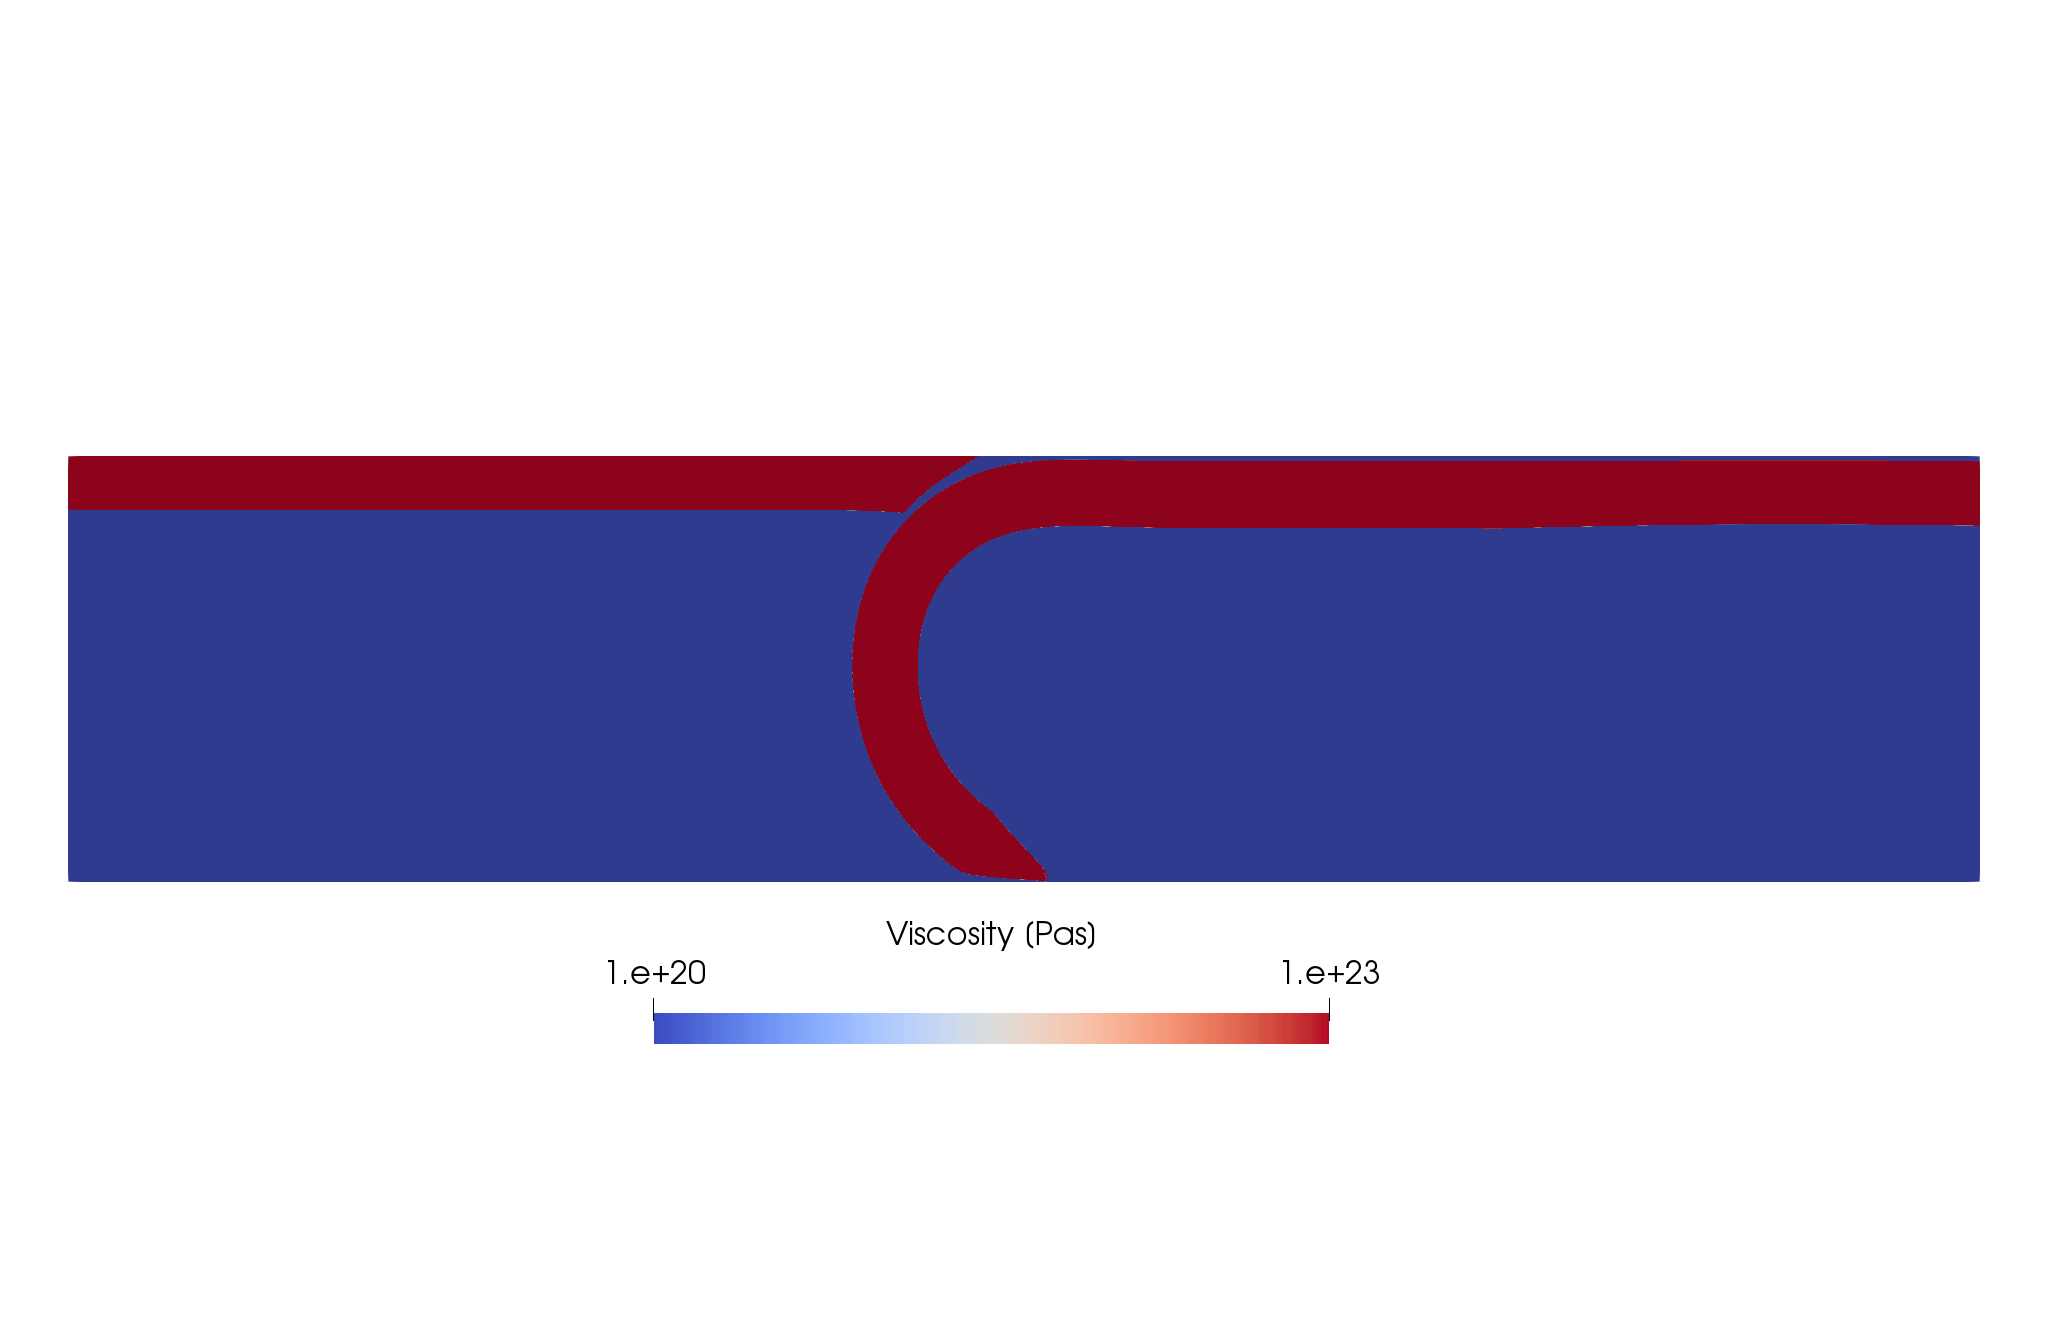
\includegraphics[width=0.6\textwidth,trim=1cm 7cm 1cm 9cm, clip=true]{Case1_visc_15My.png}
    \caption{\it Case 1 viscosity snapshots at 8 and 15 My.}
    \label{fig:QQ_case1_results}
\end{figure}
